%======================================================================
% 附录M：聚变等离子体加热、电流驱动与运行极限（注明出处）
%======================================================================
% 章标题 \appchapter{附录M：...} 由主文件发出，本文件只提供正文。
% 设计约定：这是"从物理到装置"的专题深挖，补第 10 章没有展开的加热/电流驱动/运行极限。
% 版权约定：只借鉴经典教材与文献的物理结论与公式形式，文字与数值由本书自拟并独立复算。
% 数值来源：tools/calc/appM_calc2.py（每一节的关键数字都能由它复现）。

第 10 章讲了劳森判据、点火条件与托卡马克/仿星器两条路线。但它把三件事留在了正文之外：把等离子体\textbf{加热到 10 keV}、\textbf{非感应地驱动电流}、装置\textbf{能跑到多大密度与多大比压}。本附录把这条「从物理到装置」的链条补齐。

\begin{tip}{单位错位自查}{tip-appm-units}
若你的结果与文中差一个量级，先检查四种单位错位：$\mathrm{eV}$ 与 $\mathrm{keV}$、$\mathrm{A/m^2}$ 与 $\mathrm{MA/m^2}$、$\mathrm{GHz}$ 与 $\mathrm{Hz}$、以及 $\mathrm{10^{20}\ m^{-3}}$ 这一密度单位（托卡马克文献习惯用它）。
\end{tip}


\section{加热手段全景与功率账}

聚变堆芯的功率平衡（第 10 章的零维模型）是
\begin{equation}
\frac{\diff W}{\diff t}=P_\alpha+P_{\mathrm{ext}}-P_{\mathrm{loss}},
\qquad P_\alpha=\frac15 P_{\mathrm{fus}},
\end{equation}
其中 $P_\alpha$ 是聚变产生的 $3.5\ \mathrm{MeV}$ $\alpha$ 粒子留在等离子体中的自加热功率，$P_{\mathrm{ext}}$ 是外部加热（下面五种手段之和），$P_{\mathrm{loss}}$ 是输运与辐射损失。\textbf{点火}的定义就是 $P_\alpha$ 单独撑起 $P_{\mathrm{loss}}$，即 $P_{\mathrm{ext}}\to0$。

\begin{table}[htbp]
\centering
\small
\caption{聚变等离子体的加热与电流驱动手段一览（参数区间为托卡马克量级）}
\label{tab:app-m-heating}
\begin{tabular}{@{}p{2.3cm}p{4.7cm}p{4.2cm}p{5.0cm}@{}}
\toprule
手段 & 物理机制 & 典型参数区间 & 主要限制 \\
\midrule
欧姆加热 & 等离子体电流的焦耳耗散 $P_\Omega=\eta_\parallel j^2$ & $j\sim1\ \mathrm{MA/m^2}$；$T_e\lesssim1\ \mathrm{keV}$ 有效 & $\eta_\parallel\propto T_e^{-3/2}$，温度越高越无效（见 \S M.2） \\
中性束 NBI & 高能中性原子穿入后电离、被磁场俘获 & $100\ \mathrm{keV}$--$1\ \mathrm{MeV}$，$10$--$50\ \mathrm{MW}$ & 穿透深度与效率随能量下降；须先中和（见 \S M.3） \\
离子回旋 ICRH & 少数离子在 $\omega=\omega_{ci}$ 处共振吸收 & $30$--$80\ \mathrm{MHz}$ & 天线近场、杂质产生 \\
电子回旋 ECRH & $\omega=\omega_{ce}$（或 $2\omega_{ce}$）共振 & $100$--$170\ \mathrm{GHz}$ & 局域性极强、高功率源昂贵 \\
低杂波 LHCD & 朗道共振 $v_\varphi\approx(2\text{--}3)v_{te}$ 驱动电流 & $2$--$5\ \mathrm{GHz}$ & 边缘耦合与密度窗口 \\
$\alpha$ 自加热 & $3.5\ \mathrm{MeV}$ $\alpha$ 粒子慢化 & 点火后主导 & 只有 $E_b>E_c$ 的粒子才主要加热电子（见 \S M.3） \\
\bottomrule
\end{tabular}
\end{table}

\textbf{一句话记住全表：}低温靠欧姆、中温靠束与射频、高温靠 $\alpha$ 自加热；而\textbf{电流}（不是能量）要靠束与射频非感应地驱动，这是稳态运行的关键。

{\footnotesize
\textbf{出处：}Wesson《Tokamaks》（第 4 版）加热与电流驱动相关章节。
Goldston \& Rutherford《Introduction to Plasma Physics》聚变章。
Chen 第 9--10 章。
}


\section{欧姆加热：为什么它在高温下必然失效}

环形电流在电阻等离子体中的耗散功率密度是
\begin{equation}
P_\Omega=\eta_\parallel j^2,\qquad
\eta_\parallel=5.2\times10^{-5}\,\frac{\ln\Lambda}{T_e[\mathrm{eV}]^{3/2}}\ \Omega\cdot\mathrm{m}
\label{eq:app-m-spitzer}
\end{equation}
（Spitzer 纵向电阻率；$\ln\Lambda$ 为库仑对数，见第 8 章与配套手册 L 第 8 章）。

\textbf{数字例（$T_e=1\ \mathrm{keV}$、$\ln\Lambda=17$、$j=10^6\ \mathrm{A/m^2}$）：}
\begin{align*}
\eta_\parallel&=\frac{5.2\times10^{-5}\times17}{(10^3)^{3/2}}=2.80\times10^{-8}\ \Omega\cdot\mathrm{m},\\
P_\Omega&=2.80\times10^{-8}\times(10^6)^2\approx2.8\times10^4\ \mathrm{W/m^3}=28\ \mathrm{kW/m^3}.
\end{align*}
把它与配套手册 L 第 10 章算出的 $\alpha$ 自加热功率密度 $P_\alpha\approx6.2\times10^5\ \mathrm{W/m^3}$ 相比，\textbf{差 22 倍}。这一句话就解释了为什么托卡马克必须外加加热。

\textbf{标度才是要害：}$\eta_\parallel\propto T_e^{-3/2}$，温度从 $1\ \mathrm{keV}$ 升到 $10\ \mathrm{keV}$ 时电阻率降为 $10^{-3/2}=3.2\times10^{-2}$ 倍，同电流下的欧姆功率只剩 $884\ \mathrm{W/m^3}$（附录 M.6 练习 1）。而轫致辐射与杂质辐射损失随温度上升。欧姆加热因此\textbf{只适合启动与爬升阶段}。

\textbf{另一个时间尺度：}电流在导体中扩散（趋肤）的时间为
\begin{equation}
\tau_R=\frac{\mu_0 a^2}{\eta_\parallel},
\end{equation}
$a=2\ \mathrm{m}$ 时 $\tau_R=1.26\times10^{-6}\times4/2.80\times10^{-8}\approx180\ \mathrm{s}$。它意味着\textbf{电流剖面的调整比能量约束时间慢得多}，这解释了为什么欧姆放电可以长期维持，也解释了为什么「电流一旦失控（破裂）就来不及救」（第 9 章）。

{\footnotesize
\textbf{出处：}Chen 第 5 章（扩散与电阻率）。
Fitzpatrick 第 3--4 章。
Wesson《Tokamaks》等离子体电阻相关章节。
}

\begin{warning}{把欧姆加热当成主力}{warn:m-ohm}
\textbf{误区：}「有电流就有加热，所以托卡马克不需要外加加热。」
\textbf{纠正：}欧姆功率 $\propto T_e^{-3/2}$ 而损失 $\propto T_e^{1/2}$（轫致）或更陡（输运），两者必然在某温度交叉。托卡马克的这个交叉点约在 $1$--$2\ \mathrm{keV}$，远低于聚变所需的 $10$--$20\ \mathrm{keV}$。\textbf{欧姆加热只是起步档。}
\end{warning}


\begin{figure}[htbp]
\centering
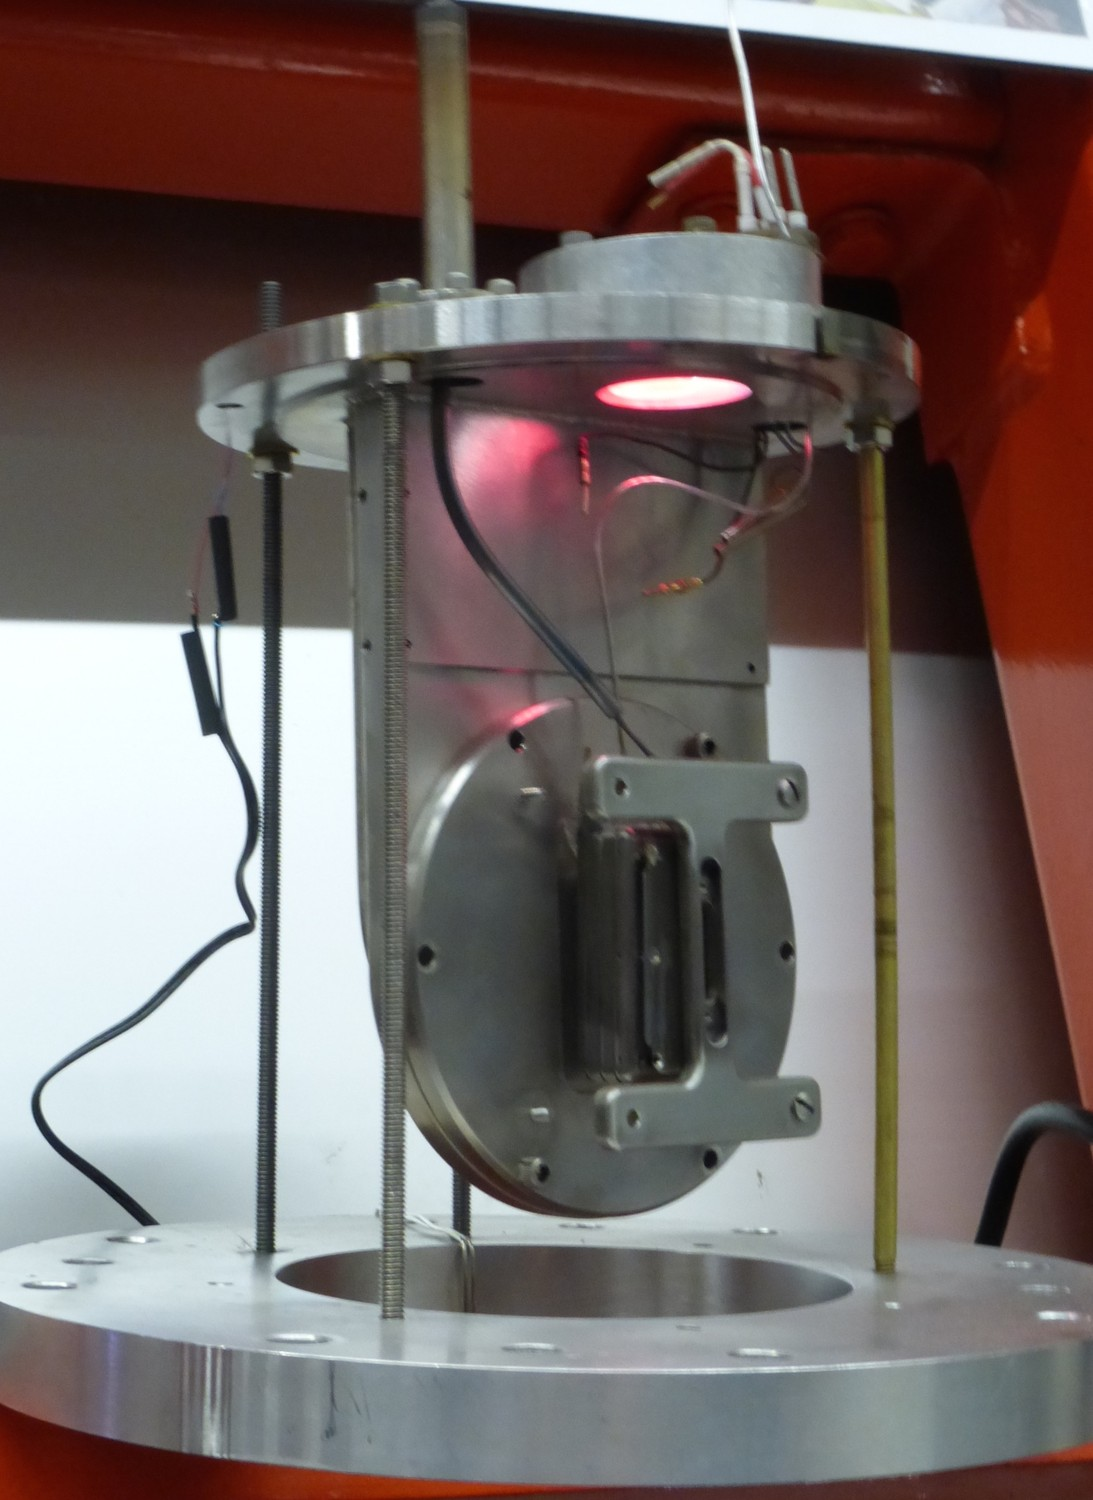
\includegraphics[width=0.65\textwidth]{../figures/ion_source_fermilab.jpg}
\caption{中性束的第一步：离子源。中性束注入先要把气体电离、引出成束，再在气体靶里中和——本节讲的束能量与穿透，起点就是照片里这台离子源。}
\label{fig:photo-appm3}
\figsource{Z22，CC BY-SA 4.0（Wikimedia Commons），链接见 figures/CREDITS.md。}
\end{figure}

\section{中性束注入：把能量「直接投进」芯部}

带电粒子出不了磁场（第 3 章），要把能量送进芯部，办法是先把离子中和成\textbf{中性原子}，让它径直穿过磁场。进入等离子体后再被电离或发生电荷交换，变成快离子被磁场俘获，这一步叫\textbf{俘获（trapping）}。

\textbf{穿透深度。}中性束强度按指数衰减
\begin{equation}
\frac{\diff I}{\diff x}=-n_e\sigma_{\mathrm{eff}}I
\quad\Longrightarrow\quad
I(x)=I_0\,e^{-x/\lambda},\qquad
\lambda=\frac{1}{n_e\sigma_{\mathrm{eff}}},
\end{equation}
其中 $\sigma_{\mathrm{eff}}$ 是把电子电离、离子电离与电荷交换合并后的等效截面，量级为 $10^{-20}\ \mathrm{m^2}$（随束能缓变）。取 $n_e=10^{20}\ \mathrm{m^{-3}}$，
\[
\lambda=\frac{1}{10^{20}\times10^{-20}}=1\ \mathrm{m},
\]
即\textbf{中性束的射程约为米级}——正好与托卡马克的尺度同量级。这是中性束能用的原因，也是它难用的原因：装置一大，束就必须更「硬」（能量更高）才能到芯部。

\textbf{束速度。}$E_b=100\ \mathrm{keV}$ 的氘束：
\[
v_b=\sqrt{\frac{2E_b}{m_D}}
=\sqrt{\frac{2\times1.60\times10^{-14}}{3.34\times10^{-27}}}
\approx3.10\times10^{6}\ \mathrm{m/s}
\]
（约 $1\%$ 光速）；$1\ \mathrm{MeV}$ 时 $v_b\approx9.79\times10^{6}\ \mathrm{m/s}$（附录 M.6 练习 2）。这个速度远大于离子热速度，所以快离子是「非热」的自由能来源，也是第 9 章里各种高能粒子驱动不稳定性（鱼骨模、阿尔芬本征模）的种子。

\textbf{慢化到哪去：临界能量。}快离子与背景电子、离子碰撞而慢化，两类碰撞的分界是\textbf{临界能量}
\begin{equation}
E_c=14.8\,T_e[\mathrm{keV}]\,A_b
\left(\frac{\sum_i n_iZ_i^2/A_i}{n_e}\right)^{2/3}\ \mathrm{keV}.
\label{eq:app-m-ecrit}
\end{equation}
对纯氘背景、$Z_i=A_i=1$，括号内为 $1/A_i=1/2$，故 $E_c=14.8\,T_eA_b(1/2)^{2/3}$：$T_e=10\ \mathrm{keV}$、氘束（$A_b=2$）时 $E_c\approx186\ \mathrm{keV}$；$T_e=1\ \mathrm{keV}$ 时 $E_c\approx18.6\ \mathrm{keV}$。

\textbf{怎么用这个结论：}
\begin{itemize}[leftmargin=1.4em]
\item $E_b>E_c$（例如 $1\ \mathrm{MeV}$ 束）：能量主要交给\textbf{电子}，加热效率高，适合把 $T_e$ 顶上去；
\item $E_b<E_c$（例如 $100\ \mathrm{keV}$ 束）：能量主要交给\textbf{离子}，且因为束离子沿磁场方向的速度分量大，\textbf{驱动电流的效率更高}；
\item 束能量不能无限提高：$E_b$ 越高，束的穿透变好但中和效率、电流驱动效率都下降，且高能离子更容易激发不稳定性——工程上在 $100\ \mathrm{keV}$--$1\ \mathrm{MeV}$ 之间取折中。
\end{itemize}

\textbf{电流驱动效率。}文献习惯用
\begin{equation}
\gamma=\frac{n_{20}\,I_{\mathrm{RF}}[\mathrm{MA}]\,R[\mathrm{m}]}{P_{\mathrm{RF}}[\mathrm{MW}]}
\end{equation}
衡量「每瓦能驱动多少电流」（$n_{20}$ 为 $10^{20}\ \mathrm{m^{-3}}$ 为单位的密度）。中性束与低杂波的典型值 $\gamma\approx0.3$：在 $R=6.2\ \mathrm{m}$ 的装置上驱动 $1\ \mathrm{MA}$，需要
\[
P_{\mathrm{RF}}=\frac{1\times1\times6.2}{0.3}\approx21\ \mathrm{MW},
\]
这正好是 ITER 量级装置辅助加热功率的数量级；相比之下电子回旋电流驱动 $\gamma\approx0.05$，同样 $1\ \mathrm{MA}$ 要 $124\ \mathrm{MW}$（附录 M.6 练习 6 会用到这个账）。

{\footnotesize
\textbf{出处：}Wesson《Tokamaks》（第 4 版）中性束注入与电流驱动章节。
Goldston \& Rutherford《Introduction to Plasma Physics》聚变章。
临界能量公式的经典形式见 Wesson 与 Stix 的综述（本书只做数量级使用，系数 $14.8$ 保留经典写法）。
}


\begin{figure}[htbp]
\centering
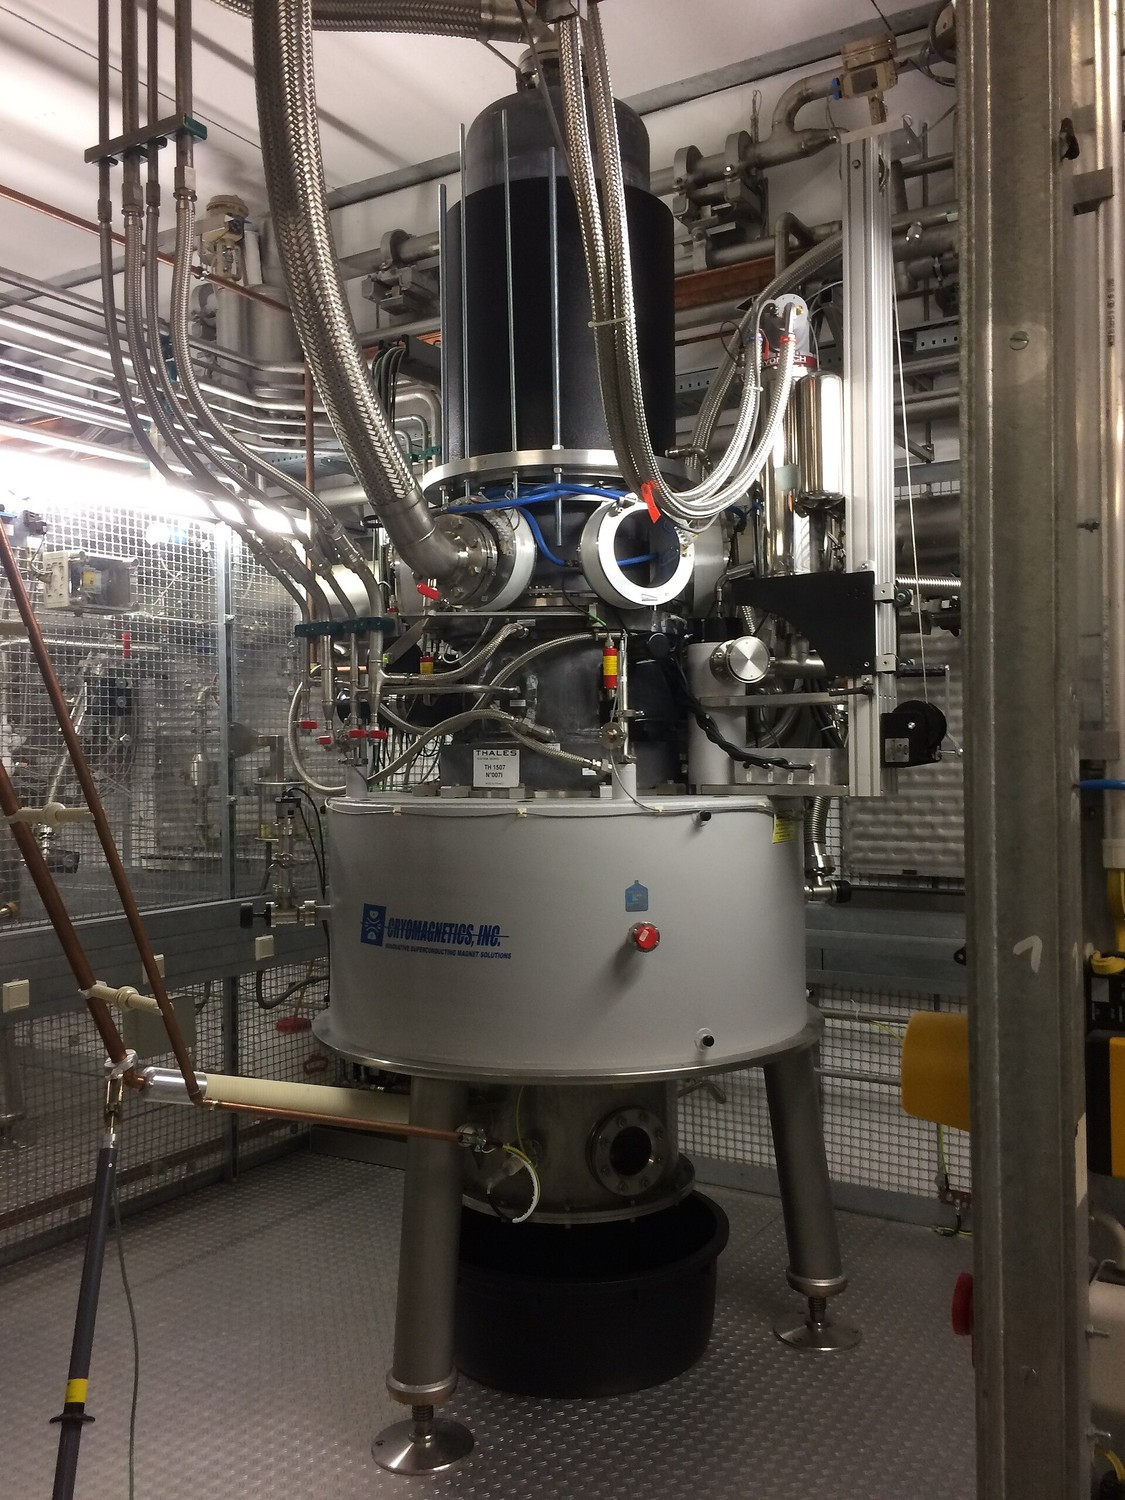
\includegraphics[width=0.67\textwidth]{../figures/gyrotron_140ghz.jpg}
\caption{射频加热三件套之一：回旋管。140 GHz、1 MW 的回旋管是 ECRH 的功率单元；加热手段的选择不只看物理，还要看这个频段能不能造出足够功率的源——本节功率账里那一列数字就是它。}
\label{fig:photo-appm2}
\figsource{Z6ehswhha5HGRTd，CC BY-SA 4.0（Wikimedia Commons），链接见 figures/CREDITS.md。}
\end{figure}

\section{射频加热三件套：ICRH、ECRH 与低杂波}

射频加热的共同逻辑是：让波在等离子体内部的某个\textbf{共振层}被吸收，从而把能量沉积在指定半径上。三种手段的区别只在「共振谁」。

\begin{table}[htbp]
\centering
\small
\caption{三种射频加热手段的共振条件与本书算例（$B_0=5.3\ \mathrm{T}$、$T_e=10\ \mathrm{keV}$）}
\label{tab:app-m-rf}
\begin{tabular}{@{}p{1.7cm}p{5.0cm}p{3.7cm}p{5.3cm}@{}}
\toprule
手段 & 共振条件 & 频率范围 & 本书算例 \\
\midrule
ICRH & $\omega=\omega_{ci}$（少数离子回旋共振） & $30$--$80\ \mathrm{MHz}$ & 氘在 $B=5.24\ \mathrm{T}$ 共振于 $40\ \mathrm{MHz}$；氢只需 $2.62\ \mathrm{T}$ \\
ECRH & $\omega=\omega_{ce}$ 或 $2\omega_{ce}$ & $100$--$170\ \mathrm{GHz}$ & $f_{ce}=28.0\ \mathrm{GHz/T}\times B$：$5.3\ \mathrm{T}$ 对应 $148\ \mathrm{GHz}$ \\
低杂波 LHCD & 朗道共振 $v_\varphi=\omega/k_\parallel\approx(2\text{--}3)v_{te}$ & $2$--$5\ \mathrm{GHz}$ & $f_{\mathrm{LH}}=\sqrt{f_{ci}f_{ce}}\approx2.45\ \mathrm{GHz}$，$\lambda_\parallel\approx5$--$7\ \mathrm{cm}$ \\
\bottomrule
\end{tabular}
\end{table}

\textbf{离子回旋共振加热（ICRH）。}由 $\omega_{ci}=qB/m_i$ 可得共振磁场
\[
B_{\mathrm{res}}=\frac{2\pi f\,m_i}{q},
\]
即\textbf{同一频率下，不同离子的共振磁场不同}。这正是「少数离子加热」的原理：在氘等离子体中掺入少量氢（或 $^3\mathrm{He}$），把频率对准\textbf{氢}的回旋层，波在氢上被强烈吸收，再通过碰撞把能量转交给氘背景。$40\ \mathrm{MHz}$ 对氘是 $5.24\ \mathrm{T}$、对氢只有 $2.62\ \mathrm{T}$（附录 M.6 会练习用电子的 $170\ \mathrm{GHz}$ 反推磁场）。

\textbf{电子回旋共振加热（ECRH）。}$\omega_{ce}=eB/m_e$，数值上
\[
\frac{f_{ce}}{B}=28.0\ \mathrm{GHz/T},
\]
所以 $B=5.3\ \mathrm{T}$ 时基频为 $148\ \mathrm{GHz}$，而 $170\ \mathrm{GHz}$ 对应 $6.07\ \mathrm{T}$。这正是 ITER（$B_0\approx5.3\ \mathrm{T}$）选 $170\ \mathrm{GHz}$ 的原因：它落在 $2\omega_{ce}$ 附近，且这个频段有成熟的兆瓦级回旋管。ECRH 的共振层极薄，因此\textbf{沉积位置最可控}，常用来抑制新经典撕裂模（第 9 章）与做局域输运实验；代价是设备昂贵、单管功率有限。

\textbf{低杂波电流驱动（LHCD）。}低杂波频率介于离子与电子回旋频率之间，
\[
f_{\mathrm{LH}}\approx\sqrt{f_{ci}f_{ce}}
=\sqrt{4.04\times10^{7}\times1.48\times10^{11}}\approx2.45\ \mathrm{GHz}.
\]
它的杀手锏是\textbf{平行相速度可调}：只要把 $k_\parallel$ 调到 $v_\varphi=\omega/k_\parallel\approx(2\text{--}3)v_{te}$，波就会通过朗道共振（第 7 章）把能量交给沿磁场方向运动的电子，从而\textbf{驱动定向电流}。取本书约定的 $v_{te}=\sqrt{2T_e/m_e}=5.93\times10^{7}\ \mathrm{m/s}$（$10\ \mathrm{keV}$）：
\[
k_\parallel=\frac{2\pi f}{v_\varphi}
=\frac{1.54\times10^{10}}{1.19\times10^{8}}\approx130\ \mathrm{m^{-1}}
\quad(\lambda_\parallel\approx4.8\ \mathrm{cm}),
\]
若取 $v_\varphi=3v_{te}$ 则 $k_\parallel\approx87\ \mathrm{m^{-1}}$（$\lambda_\parallel\approx7.3\ \mathrm{cm}$）。\textbf{厘米级的平行波长}是低杂波天线的设计难点：波导阵列的相位差必须精确可控，而边缘密度又会影响耦合。

\begin{warning}{把「共振」当成「任意位置都能加热」}{warn:m-res}
\textbf{误区：}「射频加热想加热哪里就加热哪里。」
\textbf{纠正：}共振层的位置由\textbf{磁场剖面}决定（$\omega=\omega_c(B)$ 只在某半径满足），因此波把能量沉积在哪里，取决于你选的频率与装置的磁场分布。低杂波还要额外满足 $k_\parallel$ 的朗道条件与边缘耦合窗口。\textbf{「可及性（accessibility）」与「耦合」是射频加热的两个真正的难点}，不是工程细节。
\end{warning}

{\footnotesize
\textbf{出处：}Wesson《Tokamaks》射频加热与电流驱动章节。
Lieberman \& Lichtenberg《Principles of Plasma Discharges and Materials Processing》射频鞘层与耦合相关章节（与第 11 章的天线鞘层同源）。
Chen 第 4、6 章（波的色散与共振）。
}


\section{运行极限：密度、比压与 H 模阈值}

装置不是「想加多少功率就能加多少」。托卡马克有三条被反复验证的\textbf{经验边界}，它们决定了运行空间。

\textbf{（1）Greenwald 密度极限。}用 $10^{20}\ \mathrm{m^{-3}}$ 作单位，
\begin{equation}
n_G=\frac{I_p[\mathrm{MA}]}{\pi a^2[\mathrm{m^2}]},
\label{eq:app-m-greenwald}
\end{equation}
$I_p=15\ \mathrm{MA}$、$a=2\ \mathrm{m}$ 时 $n_G\approx1.19\times10^{20}\ \mathrm{m^{-3}}$。超过它，边缘温度下降、辐射功率陡增、电流剖面收缩，最终往往以破裂收场。物理上它是「边缘辐射与输运」的结果，但\textbf{定标本身是经验的}（Greenwald 等，1988），不是从第一性原理推出的。

\textbf{（2）Troyon 比压极限。}归一化比压
\begin{equation}
\beta_N=\frac{\beta[\%]\,a[\mathrm{m}]\,B[\mathrm{T}]}{I_p[\mathrm{MA}]}
\end{equation}
的实验上限约为 $2.8$--$3.5$。以 $I_p=15\ \mathrm{MA}$、$a=2\ \mathrm{m}$、$B=5.3\ \mathrm{T}$ 为例，若 $\beta=2.5\%$，则 $\beta_N\approx1.77$，约为极限的一半。比压之所以关键，是因为聚变功率密度 $\propto\beta^2B^4$：\textbf{同样的磁场下，$\beta$ 高一点，装置就能小一圈}——这是「紧凑型托卡马克」路线的全部动机。

\textbf{（3）H 模阈值（Martin 标度）。}当加热功率超过阈值，边缘会自发形成输运垒（第 9 章湍流被剪切流抑制），约束时间约翻倍，这就是 H 模。阈值功率的经验拟合为
\begin{equation}
P_{\mathrm{LH}}=0.0488\,n_{20}^{0.717}B^{0.803}S^{0.941}\ \mathrm{MW},
\label{eq:app-m-martin}
\end{equation}
$S$ 为等离子体表面积（$\mathrm{m^2}$）。取 $n_{20}=1$、$B=5.3\ \mathrm{T}$、$S=683\ \mathrm{m^2}$ 得 $P_{\mathrm{LH}}\approx86.5\ \mathrm{MW}$；而 $n_{20}=0.5$、$B=2.5\ \mathrm{T}$、$S=100\ \mathrm{m^2}$ 的小装置只要 $4.72\ \mathrm{MW}$。\textbf{阈值随密度、磁场、尺寸都缓慢上升}（指数都小于 1），所以大装置要进入 H 模更「贵」。

\textbf{（4）自举电流与先进运行模式。}在托卡马克中，被磁场捕获的粒子（香蕉轨道，第 3 章）会通过新经典输运自动产生\textbf{自举电流}，典型占总电流的 $15\%$--$50\%$。稳态运行的条件可以粗略写成
\[
f_{\mathrm{bs}}+f_{\mathrm{CD}}\approx1,
\]
即自举电流加上外部驱动的电流要能维持全部等离子体电流。这正是低杂波与中性束如此重要的原因（见 \S M.3 的效率账）。仿星器不需要等离子体电流就能约束，在「稳态」上有天然优势（第 10 章）。

\begin{warning}{把经验定标当成物理定律}{warn:m-scale}
\textbf{误区：}「$n_G$、$\beta_N$、$P_{\mathrm{LH}}$ 是物理公式，代进去就能算出装置极限。」
\textbf{纠正：}这三条都是\textbf{多装置数据的经验拟合}：散度通常在 $\pm30\%$ 甚至更大，且不同装置之间还有系统偏差（例如金属壁、偏滤器几何都会改变密度极限）。它们的正确用法是\textbf{估计数量级与设计余量}，而不是当作不可违反的定律。本书引用它们时一律标注「经验标度」。
\end{warning}

{\footnotesize
\textbf{出处：}Wesson《Tokamaks》运行极限与 H 模章节。
Greenwald 等（1988）密度极限。
Troyon 等（1984）比压极限。
Martin 等（2008）H 模阈值标度。完整书目见附录 E 与配套手册 J。
}


\section{六道估算练习（含答案）}

下面六题只用本附录与第 10 章的公式，每题都对应上面某一个小节。建议先合上书自己算，再看答案。

\begin{enumerate}[leftmargin=1.6em,itemsep=2pt]

\item \textbf{（欧姆加热的失效速度）}取 $\ln\Lambda=17$、$j=10^6\ \mathrm{A/m^2}$，求 $T_e=10\ \mathrm{keV}$ 时的 $\eta_\parallel$ 与欧姆功率密度，并与 $1\ \mathrm{keV}$ 时的 $28\ \mathrm{kW/m^3}$ 比较；再与同一温度的 $\alpha$ 自加热功率密度 $6.2\times10^{5}\ \mathrm{W/m^3}$ 比较。

\textbf{答案：}$\eta_\parallel=5.2\times10^{-5}\times17/(10^4)^{3/2}=8.84\times10^{-10}\ \Omega\cdot\mathrm{m}$，
$P_\Omega=8.84\times10^{-10}\times10^{12}=884\ \mathrm{W/m^3}$。
比 $1\ \mathrm{keV}$ 时小 $10^{3/2}=32$ 倍（$\eta\propto T_e^{-3/2}$）；比 $\alpha$ 自加热小约 $700$ 倍。
\textbf{结论：}$10\ \mathrm{keV}$ 时欧姆加热连 $\alpha$ 自加热的千分之一都不到，「高温靠自加热」是必然，不是选择。

\item \textbf{（中性束的速度与射程）}$1\ \mathrm{MeV}$ 氘束的速度是多少？如果等效截面 $\sigma_{\mathrm{eff}}$ 不变，射程会变成 $100\ \mathrm{keV}$ 束的几倍？

\textbf{答案：}$v_b=\sqrt{2E_b/m_D}=\sqrt{2\times1.60\times10^{-13}/3.34\times10^{-27}}\approx9.79\times10^{6}\ \mathrm{m/s}$（约 $3\%$ 光速），是 $100\ \mathrm{keV}$ 束（$3.10\times10^{6}\ \mathrm{m/s}$）的 $\sqrt{10}\approx3.2$ 倍。
\textbf{但射程不变}：$\lambda=1/(n_e\sigma_{\mathrm{eff}})$（$\sigma_{\mathrm{eff}}$ 保持不变时），仍是 $1\ \mathrm{m}$。
真正的依赖在于 $\sigma_{\mathrm{eff}}$ 随能量\textbf{缓慢下降}（电离截面大致按 $v^{-1}$ 到 $v^{-0.5}$ 衰减），所以射程随能量只是缓慢增长。\textbf{想靠提高束能线性地提高穿透深度是行不通的}。提高束能的主要好处是慢化时间变长、快离子能「活」得更久。

\item \textbf{（ECRH 的共振磁场）}电子回旋加热常用的 $170\ \mathrm{GHz}$ 对应多大的磁场？若装置磁场是 $5.3\ \mathrm{T}$，基频共振在什么频率？

\textbf{答案：}$B_{\mathrm{res}}=2\pi f m_e/e=2\pi\times1.70\times10^{11}\times9.11\times10^{-31}/1.60\times10^{-19}\approx6.07\ \mathrm{T}$。
$5.3\ \mathrm{T}$ 时 $f_{ce}=28.0\ \mathrm{GHz/T}\times5.3\ \mathrm{T}\approx148\ \mathrm{GHz}$——所以 ITER 的 $170\ \mathrm{GHz}$ 系统工作在 $2\omega_{ce}$ 附近（共振层位置由磁场剖面决定）。

\item \textbf{（低杂波的平行波长）}$10\ \mathrm{keV}$ 的电子，$v_{te}=\sqrt{2T_e/m_e}=5.93\times10^{7}\ \mathrm{m/s}$。若 $2.45\ \mathrm{GHz}$ 的低杂波要满足 $v_\varphi=3v_{te}$，平行波长是多少？为什么必须做到厘米级？

\textbf{答案：}$v_\varphi=1.78\times10^{8}\ \mathrm{m/s}$，
$\lambda_\parallel=2\pi v_\varphi/\omega=v_\varphi/f=1.78\times10^{8}/2.45\times10^{9}\approx7.3\ \mathrm{cm}$。
必须做到厘米级（$k_\parallel$ 为几十到几百 $\mathrm{m^{-1}}$），是因为朗道共振要求 $v_\varphi=\omega/k_\parallel$ 落在电子热速度的 $2$--$3$ 倍这个窄窗口内。频率固定时，\textbf{只有 $k_\parallel$ 足够大}才能把相速度压到电子热速度量级。这也是低杂波天线必须用波导阵列精确控制相位的原因。

\item \textbf{（密度极限与诊断）}取 $I_p=15\ \mathrm{MA}$、$a=2\ \mathrm{m}$，求 Greenwald 密度与对应的等离子体频率；$2.45\ \mathrm{GHz}$ 的干涉仪能测这个密度吗？

\textbf{答案：}$n_G=15/(\pi\times4)\approx1.19\times10^{20}\ \mathrm{m^{-3}}$；
$f_{pe}=8.98\times10^{9}\sqrt{n_e/10^{18}}\approx9.8\times10^{10}\ \mathrm{Hz}=98\ \mathrm{GHz}$。
不能：$2.45\ \mathrm{GHz}$ 的截止密度只有 $n_c\approx7.4\times10^{16}\ \mathrm{m^{-3}}$（配套手册 L 第 6 章），比 $n_G$ 低约 $1600$ 倍，波根本进不去。要测这个密度必须用 $100\ \mathrm{GHz}$ 量级（工程上用 $140\ \mathrm{GHz}$ 干涉仪）。

\item \textbf{（功率账与点火距离）}用配套手册 L 第 10 章的堆芯数字（$P_{\mathrm{fus}}=3.1\times10^{6}\ \mathrm{W/m^3}$，$P_\alpha=P_{\mathrm{fus}}/5$）。若损失功率是 $P_{\mathrm{loss}}=1.2P_\alpha$，需要多少外部加热功率密度？折算到 $V\approx840\ \mathrm{m^3}$ 的装置是多少兆瓦？

\textbf{答案：}$P_\alpha=6.2\times10^{5}\ \mathrm{W/m^3}$，
$P_{\mathrm{ext}}=P_{\mathrm{loss}}-P_\alpha=0.2P_\alpha\approx1.24\times10^{5}\ \mathrm{W/m^3}$，
折合 $P_{\mathrm{ext}}V\approx1.24\times10^{5}\times840\approx1.04\times10^{8}\ \mathrm{W}$，即 $100\ \mathrm{MW}$ 量级——与 ITER 的辅助加热（$73\ \mathrm{MW}$）同量级。
\textbf{注意口径：}这里「$P_{\mathrm{loss}}=1.2P_\alpha$」是假设，功率密度与体积两处数量级误差会相乘。这个结果只用于\textbf{判断「离点火还有多远」}：需要百兆瓦级辅助加热的装置，正好处在「$\alpha$ 自加热即将接管」的门槛附近。

\end{enumerate}

\begin{tip}{与配套手册 L 串联}{tip-appm-chain}
把这六题与配套手册 L 第 10 章的六道题连起来做，就是一条完整的「聚变工程量级链」。先算 $P_{\mathrm{fus}}$，再算 $\tau_E$ 门槛，再算加热与电流驱动的功率，最后用 $n_G$、$\beta_N$、$P_{\mathrm{LH}}$ 检查装置能不能跑到那个工作点。
\end{tip}


\section{来源、分级与版权说明}

\begingroup\small
本附录的数字都可以用 \texttt{tools/\allowbreak{}calc/\allowbreak{}appM\_calc.py} 重算一遍。
\label{sec:app-m-source}

{\small
\begin{longtable}{@{}p{1.5cm}p{5.2cm}p{5.3cm}p{3.6cm}@{}}
\caption{附录 M 各节的借鉴来源与独立性说明（与配套手册 J 的逐章对照表、L 的题库来源表配套使用）}\label{tab:app-m-source}\\
\toprule
本书节 & 借鉴的教材与文献 & 借鉴的内容（不是文字） & 独立性说明 \\
\midrule
\endfirsthead
\toprule
本书节 & 借鉴的教材与文献 & 借鉴的内容（不是文字） & 独立性说明 \\
\midrule
\endhead
\bottomrule
\endlastfoot
M.1--M.2 & Chen 第 5 章；Fitzpatrick 第 3--4 章；Wesson《Tokamaks》（第 4 版） & 欧姆加热的地位、Spitzer 纵向电阻率、电流扩散时间 $\tau_R$ & 公式用经典形式，全部数值由 \texttt{appM\_{}calc2.py} 复算 \\
M.3 & Wesson《Tokamaks》中性束与电流驱动章；Goldston \& Rutherford 聚变章 & 中性束的电离/俘获图像、衰减长度、临界能量 $E_c$、电流驱动效率 $\gamma$ 的定义 & $E_c$ 保留经典系数 $14.8$；速度、射程与功率账均自算 \\
M.4 & Wesson 射频加热章；Lieberman \& Lichtenberg（射频鞘层与耦合）；Chen 第 4、6 章 & ICRH/ECRH/LHCD 的共振条件、少数离子加热原理、$f_{\mathrm{LH}}\approx\sqrt{f_{ci}f_{ce}}$ & 共振磁场、$k_\parallel$、$\lambda_\parallel$ 等算例均自算 \\
M.5 & Wesson 运行极限章；Greenwald 等（1988）；Troyon 等（1984）；Martin 等（2008） & Greenwald 密度极限、Troyon 比压极限、H 模阈值标度、自举电流概念 & 三条标度均标注为\textbf{经验拟合}并给出散度；算例数值自算 \\
M.6 & 本书自拟 & 六道估算练习 & 题目、参数与答案全部自拟，答案已在正文中给出可复算过程 \\
\end{longtable}
}

\textbf{版权与独立性声明：}
\begin{itemize}
\item 上表的「借鉴」仅指\textbf{物理内容、公式形式与结论的组织方式}（例如「用欧姆功率与 $\alpha$ 自加热对比说明高温加热的必要性」这类公认的讲法）；
\item 本附录的\textbf{文字表述、算例参数与全部数值}均由本书自拟，并可用仓库脚本 \texttt{appM\_{}calc2.py} 或手算逐条复现（正文保留三位有效数字）；
\item 经验标度律（Greenwald、Troyon、Martin）的\textbf{原始出处按作者与年份标注}；
\item 本附录\textbf{不复制}任何教材或文献的题目原文、解答、图表与数据表，引用它们只为说明物理结论的来源。
\end{itemize}

\begin{tip}{下一步}{tip-appm-next}
附录 M 是「从物理到装置」的最后一环：把这里的功率账、运行极限与第 10 章的劳森判据拼在一起，你就能对一个聚变装置做\textbf{完整的一次量级评估}。若想继续深入，配套手册 J 给出了 Wesson 与 Freidberg 的入口。
\end{tip}
\endgroup
